\chapter[SCP-001 好孩子]{
    SCP-001 The Great Hippo (feat. Peppersghost)  - A Good Boy  \\
    SCP-001 好孩子
}

\label{chap:SCP-001.a.good.boy}

\definecolor{ftwoftwoctwo}{HTML}{f2f2c2}

\begin{tcolorbox}[
    enhanced standard,
    hbox,
    colback=ftwoftwoctwo,
    watermark graphics=images/SCP-001-a-good-boy-watermark.png,
    watermark overzoom=0.7,
    watermark opacity=1,
    center,
    before upper=\begin{varwidth}{0.9\linewidth},
        after upper=\end{varwidth},
]
\begin{minipage}[c]{0.2\linewidth}
    
\includegraphics[width=0.8\linewidth]{images/SCP-001-a-good-boy.png}
\end{minipage}
\begin{minipage}[c]{0.8\linewidth}
    
\g{\bb{注:下附档案只作为历史性参考。}}\\

\bb{这个档案已被上锁并封存。其中的资讯可能不正确,或不能反映最新的可获取数据。}\\

\bb{如果您希望编辑此档案或对其状况有任何疑问,请联系记录与信息安全管理部或寄电邮给您的IntSCPFN伺服器管理员。}\\

\bb{— Maria Jones,记录与信息安全管理部主任}\\
\end{minipage}
\end{tcolorbox}

\hr

\g{\bb{项目编号:} SCP-001-EX \hfill \tred{\bb{0\slash 001级}}}

\g{\bb{项目等级:} Explained \hfill \tred{\bb{已解密}}}

\hr

\begin{figure}[H]
    \centering
    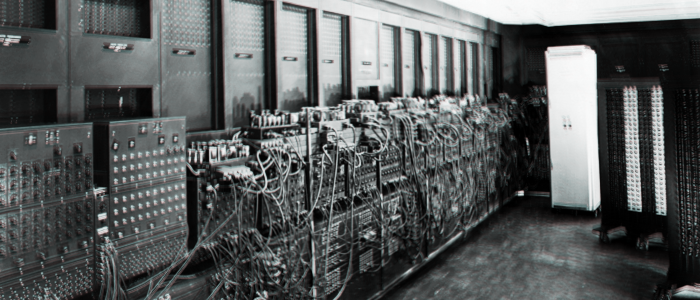
\includegraphics[width=\linewidth]{images/SCP-001-a-good-boy-2.png}
    \caption*{ERZATZ AK9型运算引擎(约1956年)}
\end{figure}

\hr

\bb{特殊收容措施:} SCP-001须保存在Site-5的一间经瞬态电磁辐射标准认证\footnote{瞬态电磁辐射标准(TEMPEST)为北大西洋公约组织规定的一种电磁波放射防护(EMSEC)认证,即隔离仪器和\slash 或建筑结构以防止资料以电磁波放射或声发射等形式泄漏。}之收容间内。不少于四名IntSCPFN\footnote{国际SCP基金会网路(IntSCPFN)是为了保持基金会收容措施相关资讯在所有站点、设施与国际间之同步而建立的全球性网路。}技术人员必须在现场以提供技术支援,并每日维护所有连接至SCP-001的无线传输组件。基金会下辖所有的大型站点、设施和行政大楼内须保持有至少两台电传打字机连接至IntSCPFN网路,以接收紧急通报及收容失效的相关预防指示。任何情况下都不允许终止SCP-001的运行或将其与IntSCPFN伺服器中断连结。

由SCP-001所预测的项目报告将转送至记录与信息安全管理部进行分析与审查。每一份报告都将安排一名记录与信息安全管理部的四级人员,其负责评估被预测项目所造成的立即性威胁、创造一个可靠的背景故事以解释基金会如何发现此项目,并安排一名收容主任\footnote{收容主任为收容指挥系统(CCS,与项目进行首次接触时的指挥系统模型)的成员之一。收容指挥系统设立于1945年,为基金会内外数个机关单位间组织的等级制度,促使成员间的协同合作以安全获取并收容异常项目。}以调查、构思与执行收容策略。所有SCP-001所建议或产生的收容措施必须取得O5议会投票过半通过后方得以施行。

\bb{描述:} SCP-001即ERZATZ AK9型运算引擎\footnote{ERZATZ AK9型运算引擎是一台多功能的数码计算机,符合图灵完备性标准。},于1955年由基金会建造而成,目的在于提供尚未被发现之异常项目的地点与性质之预测性分析;其原理乃是将过去已知的项目地点与性质等训练资料集,透过多层感知器\footnote{多层感知器(MLP)是一种前向结构的运算系统,其含有不少于三层之节点:输入层(顶层)、一至多个隐藏层(中间层)及输出层(底层);每一层之节点都与其下一层之每一个节点间以箭号相连。感知器自其输入层接受一个数值后,其沿着路径与方向在感知器中逐层移动与变换,直到其最终产生一个输出值。}进行分析。多层感知器的运用之所以能够成为一个有效的预测模型,归功于普罗米修斯实验室(基金会分析学部于1951年将其并入部门)的几名前员工所研发的高级反向传播算法。

1959年,SCP-001被假定可以经由预测性的文本协助加强Euclid和Keter级项目的收容措施。数以千计的收容措施草案(包含过去或当前的版本)依其表现权重(尤重比较当前版本与其他旧版本间收容成效落差)后,被输入SCP-001作为训练资料集。此后由SCP-001所建议修订之收容措施一致的降低了收容失效发生的机率,甚至影响了许多并无关联之项目。在许多状况下,这些修订亦导致了项目异常行为的消失。

\bb{附录001.1:} 文件

\newpage

\begin{whitebox}

\bb{315D27}

\cl{\bu{ERZATZ提案摘要}}

\bb{输入:\\
\phantom{空白}\hyperref[chap:SCP-1773]{SCP-1773}的收容措施}

\bb{输出:\\
\phantom{空白}“每两周一次将尘土置于它们之中,以捐赠门厅更加美丽的功能。”}

\bb{提案:\\
\phantom{空白}“修订SCP-1773的收容措施,每两周在其容器中加入十克的灰尘。”(O5-01)}

\cl{\bb{议会投票摘要:}}

\begin{longtable}{|c|c|c|}
\multicolumn{1}{c}{\bb{赞成}} & \multicolumn{1}{c}{\bb{反对}} & \multicolumn{1}{c}{\bb{弃权}}\\
\hline
\endhead
\hline
\multicolumn{3}{r}{\small{接下页}}
\endfoot
\hline
\endlastfoot
\bb{O5-01} & \bb{O5-02} & \bb{O5-03}\\
\bb{O5-04} &  & \bb{O5-13}\\
\bb{O5-05} &  & \\
\bb{O5-06} &  & \\
\bb{O5-07} &  & \\
\bb{O5-08} &  & \\
\bb{O5-09} &  & \\
\bb{O5-10} &  & \\
\bb{O5-11} &  & \\
\bb{O5-12} &  & \\
\hline
\end{longtable}

\begin{longtable}{|c|}
\multicolumn{1}{c}{\bb{结果}}\\
\hline
\endhead
\hline\multicolumn{1}{r}{\small{接下页}}
\endfoot
\hline
\endlastfoot
\bb{\green{通过}}\\
\hline
\end{longtable}

\bb{附注:\\
\phantom{空白}SCP-1773的行为与特性并未被观察到有任何变化。然而,负责\hyperref[chap:SCP-1384]{SCP-1384}的研究员回报了项目于二月15日下午3:22时(即SCP-1773之文件更新时间)向后走了三步。}

\end{whitebox}

\begin{whitebox}

\bb{111H43}

\cl{\bu{ERZATZ提案摘要}}

\bb{\uu{输入}:\\
\phantom{空白}\hyperref[chap:SCP-3034]{SCP-3034}的收容措施}

\bb{\uu{输出}:\\
\phantom{空白}“不论其是否显然知晓基金会的管理失当,任何小型且只为孩童的人类都将不会被授予一级安保权限。”}

\bb{\uu{提案}:\\
\phantom{空白}“修订SCP-3034的收容措施,明确的禁止孩童接近站点。”(O5-04)}

\cl{\bb{\uu{议会投票摘要}:}}

\begin{longtable}{|c|c|c|}
\multicolumn{1}{c}{\bb{赞成}} & \multicolumn{1}{c}{\bb{反对}} & \multicolumn{1}{c}{\bb{弃权}}\\
\hline
\endhead
\hline\multicolumn{3}{r}{\small{接下页}}
\endfoot
\hline
\endlastfoot
\bb{O5-04} & \bb{O5-02} & \bb{O5-01}\\
\bb{O5-05} &  & \bb{O5-03}\\
\bb{O5-06} &  & \bb{O5-13}\\
\bb{O5-07} &  & \\
\bb{O5-08} &  & \\
\bb{O5-09} &  & \\
\bb{O5-10} &  & \\
\bb{O5-11} &  & \\
\bb{O5-12} &  & \\
\hline
\end{longtable}

\begin{longtable}{|c|}
\multicolumn{1}{c}{\bb{结果}}\\
\hline
\endhead
\hline\multicolumn{1}{r}{\small{接下页}}
\endfoot
\hline
\endlastfoot
\bb{\green{通过}}\\
\hline
\end{longtable}

\bb{\uu{附注}:\\
\phantom{空白}未观察到任何变化。}

\end{whitebox}

\begin{whitebox}

\bb{672C91}

\cl{\bu{ERZATZ提案摘要}}

\bb{输入:\\
\phantom{空白}无}

\bb{输出:\\
\phantom{空白}“Site-13将现于行星他处,包围作画于空白石板上的白种男人与在他们血液中流淌的枪声。”}

\bb{提案:\\
\phantom{空白}由于毫无基金会建造Site-13的证据,O5议会无法自此资料中推论出任何建议的行动。}

\begin{longtable}{|c|}
\multicolumn{1}{c}{\bb{结果}}\\
\hline
\endhead
\hline\multicolumn{1}{r}{\small{接下页}}
\endfoot
\hline
\endlastfoot
\bb{\tred{否决}}\\
\hline
\end{longtable}

\bb{附注:\\
\phantom{空白}提出此提案之五天后,\hyperref[chap:SCP-1730]{SCP-1730}出现。}

\end{whitebox}

\begin{whitebox}

\bb{954E36}

\cl{\bu{ERZATZ提案摘要}}

\bb{输入:\\
\phantom{空白}\hyperref[chap:SCP-2170]{SCP-2170}的收容措施}

\bb{输出:\\
\phantom{空白}“对红唇男子持有开放襟怀的人们,永远不会知晓如肿瘤般许可的灼热惊喜。总是,爱小丑。”}

\bb{提案:\\
\phantom{空白}“修订SCP-2170的收容措施,只允许对小丑或相关媒体内容感到强烈喜爱的人员接触项目。”(O5-01)}

\cl{\bb{议会投票摘要:}}

\begin{longtable}{|c|c|c|}
\multicolumn{1}{c}{\bb{赞成}} & \multicolumn{1}{c}{\bb{反对}} & \multicolumn{1}{c}{\bb{弃权}}\\
\hline
\endhead
\hline\multicolumn{3}{r}{\small{接下页}}
\endfoot
\hline
\endlastfoot
\bb{O5-01} & \bb{O5-02} & \\
\bb{O5-03} & \bb{O5-04} & \\
\bb{O5-07} & \bb{O5-05} & \\
\bb{O5-09} & \bb{O5-06} & \\
\bb{O5-10} & \bb{O5-08} & \\
\bb{O5-12} & \bb{O5-11} & \\
\bb{O5-13} &  & \\
\hline
\end{longtable}

\begin{longtable}{|c|}
\multicolumn{1}{c}{\bb{结果}}\\
\hline
\endhead
\hline\multicolumn{1}{r}{\small{接下页}}
\endfoot
\hline
\endlastfoot
\bb{\green{通过}}\\
\hline
\end{longtable}

\bb{附注:\\
\phantom{空白}对小丑及相关媒体内容表现出正向联想的人员被发现对于SCP-2170的异常特性拥有较高的抗性。更多基于小丑的模因疫苗接种研究待议中。}

\end{whitebox}

\begin{whitebox}

\bb{149B22}

\cl{\bu{ERZATZ提案摘要}}

\bb{输入:\\
\phantom{空白}无}

\bb{输出:\\
\phantom{空白}“我看见铝质士兵的脏器自口中挤出。我看见它们被九十五(95)号站点里一直研究着它们的人类有效的歼灭。我看见一片寒冷,整个门厅里它们只是看着自己的尸体以示自己拥有智能。”}

\bb{提案:\\
\phantom{空白}“将Site-95的安保人员数量加倍,并令所有在现场的机动特遣队进入立即待命状态。”(O5-05)}

\cl{\bb{议会投票摘要:}}

\begin{longtable}{|c|c|c|}
\multicolumn{1}{c}{\bb{赞成}} & \multicolumn{1}{c}{\bb{反对}} & \multicolumn{1}{c}{\bb{弃权}}\\
\hline
\endhead
\hline\multicolumn{3}{r}{\small{接下页}}
\endfoot
\hline
\endlastfoot
\bb{O5-01} &  & \bb{O5-02}\\
\bb{O5-03} &  & \bb{O5-08}\\
\bb{O5-04} &  & \bb{O5-13}\\
\bb{O5-05} &  & \\
\bb{O5-06} &  & \\
\bb{O5-07} &  & \\
\bb{O5-09} &  & \\
\bb{O5-10} &  & \\
\bb{O5-11} &  & \\
\bb{O5-12} &  & \\
\hline
\end{longtable}

\begin{longtable}{|c|}
\multicolumn{1}{c}{\bb{结果}}\\
\hline
\endhead
\hline\multicolumn{1}{r}{\small{接下页}}
\endfoot
\hline
\endlastfoot
\bb{\green{通过}}\\
\hline
\end{longtable}

\bb{附注:\\
\phantom{空白}提案通过的三天后,一个排的超常科技改造\hyperref[chap:SCP-3033]{士兵}在一名\hyperref[chap:]{分裂者}特工的带领下攻击了Site-95。事后证明,事先增加的现场安保人员对于击退此次攻击是至关重要的。}

\end{whitebox}

\definecolor{dffffthree}{HTML}{DFFFF3}
\newtcolorbox{greenbox}[1][]{
    enhanced standard,
    colback=dffffthree,
    colframe=black,
    boxrule=0.5pt,
    watermark graphics=images/SCP-001-a-good-boy-watermark.png,
    watermark overzoom=0.7,
    watermark opacity=1,
}

\begin{greenbox}

\cl{\bu{O5议会提案摘要}}

\bb{提案:\\
\phantom{空白}“利用ERTZATZ AK9型运算引擎预测威胁和收容失效之能力,建立多站点早期预警系统。”(O5-05)}

\cl{\bb{议会投票摘要:}}

\begin{longtable}{|c|c|c|}
\multicolumn{1}{c}{\bb{赞成}} & \multicolumn{1}{c}{\bb{反对}} & \multicolumn{1}{c}{\bb{弃权}}\\
\hline
\endhead
\hline\multicolumn{3}{r}{\small{接下页}}
\endfoot
\hline
\endlastfoot
\bb{O5-03} & \bb{O5-01} & \\
\bb{O5-05} & \bb{O5-02} & \\
\bb{O5-06} & \bb{O5-04} & \\
\bb{O5-07} & \bb{O5-08} & \\
\bb{O5-10} & \bb{O5-09} & \\
\bb{O5-12} & \bb{O5-11} & \\
\bb{O5-13} &  & \\
\hline
\end{longtable}

\begin{longtable}{|c|}
\multicolumn{1}{c}{\bb{结果}}\\
\hline
\endhead
\hline\multicolumn{1}{r}{\small{接下页}}
\endfoot
\hline
\endlastfoot
\bb{\green{通过}}\\
\hline
\end{longtable}

\bb{附注:\\
\phantom{空白}提案通过三个月后,多站点自动紧急电报分配系统(MAYDAY)被设立。其仰赖人类对ERTZATZ AK9型运算引擎所输出之收容失效预测信息的翻译,并从中规画预防性措施。}

\end{greenbox}

\begin{whitebox}

\bb{229K36}

\cl{\bu{ERZATZ提案摘要}}

\bb{输入:\\
\phantom{空白}无}

\bb{输出:\\
\phantom{空白}“统一的收容措施容器将可以大幅增加其保障。五乘五乘五(5x5x5)(五x五x5)的容器自内部使其服从,其他数值也是受保障的。”}

\bb{提案:\\
\phantom{空白}“修订数个高危险性项目之收容措施并规定精确的收容间尺寸。在三个月内全面调查收容措施,以判定其效果是否有任何增加。”(O5-03)}

\cl{\bb{议会投票摘要:}}

\begin{longtable}{|c|c|c|}
\multicolumn{1}{c}{\bb{赞成}} & \multicolumn{1}{c}{\bb{反对}} & \multicolumn{1}{c}{\bb{弃权}}\\
\hline
\endhead
\hline\multicolumn{3}{r}{\small{接下页}}
\endfoot
\hline
\endlastfoot
\bb{O5-03} & \bb{O5-01} & \bb{O5-13}\\
\bb{O5-05} & \bb{O5-02} & \bb{O5-08}\\
\bb{O5-06} & \bb{O5-04} & \\
\bb{O5-07} & \bb{O5-09} & \\
\bb{O5-10} & \bb{O5-11} & \\
\bb{O5-12} &  & \\
\hline
\end{longtable}

\begin{longtable}{|c|}
\multicolumn{1}{c}{\bb{结果}}\\
\hline
\endhead
\hline\multicolumn{1}{r}{\small{接下页}}
\endfoot
\hline
\endlastfoot
\bb{\green{通过}}\\
\hline
\end{longtable}

\bb{附注:\\
\phantom{空白}全面调查后发现相关项目之严重性均大幅下降,由它们所造成的收容失效数量亦明显降低。上述的状况在收容间的尺寸被规定为五的倍数时最为显著。}

\end{whitebox}

\begin{whitebox}

\bb{713D27}

\cl{\bu{ERZATZ提案摘要}}

\bb{输入:\\
\phantom{空白}\hyperref[chap:SCP-1459]{SCP-1459}的收容措施}

\bb{输出:\\
\phantom{空白}“坏孩子。不要停。不要停。不要停。不要停。不要停。不要停。不要停。不要停。不要停。不要停。不要停。不要停。不要停。不要停。不要停。不要停。不要停。不要停。不要停。不要停。不要停。不要停。不要停。不要停。不要停。不要停。不要停。不要停。不要停。不要停。不要停。不要停。不要停。不要停。不要停。不要停。不要停。不要停。不要停。不要停。不要停。不要…”\\
\phantom{空白}{[}资料编辑以缩短长度]}

\bb{提案:\\
\phantom{空白}“无限期继续对SCP-1459进行测试。”(O5-05)}

\cl{\bb{议会投票摘要:}}

\begin{longtable}{|c|c|c|}
\multicolumn{1}{c}{\bb{赞成}} & \multicolumn{1}{c}{\bb{反对}} & \multicolumn{1}{c}{\bb{弃权}}\\
\hline
\endhead
\hline\multicolumn{3}{r}{\small{接下页}}
\endfoot
\hline
\endlastfoot
\bb{O5-03} & \bb{O5-01} & \\
\bb{O5-04} & \bb{O5-02} & \\
\bb{O5-05} & \bb{O5-06} & \\
\bb{O5-07} & \bb{O5-08} & \\
\bb{O5-09} & \bb{O5-11} & \\
\bb{O5-10} &  & \\
\bb{O5-12} &  & \\
\bb{O5-13} &  & \\
\hline
\end{longtable}

\begin{longtable}{|c|}
\multicolumn{1}{c}{\bb{结果}}\\
\hline
\endhead
\hline\multicolumn{1}{r}{\small{接下页}}
\endfoot
\hline
\endlastfoot
\green{\bb{通过}}\\
\hline
\end{longtable}

\bb{附注:\\
\phantom{空白}对\hyperref[chap:SCP-1459]{SCP-1459}的测试将无限期的持续下去。}

\end{whitebox}

\definecolor{ffdsixnineseven}{HTML}{FFD697}
\begin{whitebox}[colback=ffdsixnineseven]

\cl{\bu{全站紧急公告}}

\bb{优先等级:EPSILON}

\bb{地点:Site-114}

\bb{\phantom{空白}所有的地下室应被以水反复不断淹没自身。如此这般便能遏止鸟猿排卵。它们会变成好孩子。立刻让它们成为好孩子。}

\bb{附注:\\
\phantom{空白}此一公告发布后大约五小时,一个\hyperref[chap:SCP-3199]{SCP-3199}实体突破收容。站点人员将Site-114地下空间以水淹没,致使此实体进入惰性状态。此一发现已被记录至SCP-3199的档案中。}

\end{whitebox}

\begin{whitebox}
    
\bb{821C95}

\cl{\bu{ERZATZ提案摘要}}

\bb{输入:\\
\phantom{空白}\hyperref[chap:SCP-2717]{SCP-2717}的收容措施}

\bb{输出:\\
\phantom{空白}“两(2)个样本将成为目标。两个人类在进入项目的体内前,必须由骨和肉制成。他们将不会再离开,由他们去吧。”}

\bb{提案:\\
\phantom{空白}“修订SCP-2717的收容措施,以确保至少两名参与其中的D级人员在进入其生物质内后无法被回收。”(O5-04)}

\cl{\bb{议会投票摘要:}}

\begin{longtable}{|c|c|c|}
\multicolumn{1}{c}{\bb{赞成}} & \multicolumn{1}{c}{\bb{反对}} & \multicolumn{1}{c}{\bb{弃权}}\\
\hline
\endhead
\hline\multicolumn{3}{r}{\small{接下页}}
\endfoot
\hline
\endlastfoot
\bb{O5-04} & \bb{O5-02} & \bb{O5-01}\\
\bb{O5-09} & \bb{O5-03} & \bb{O5-13}\\
\bb{O5-12} & \bb{O5-05} & \\
 & \bb{O5-06} & \\
 & \bb{O5-07} & \\
 & \bb{O5-08} & \\
 & \bb{O5-10} & \\
 & \bb{O5-11} & \\
 \hline
\end{longtable}

\begin{longtable}{|c|}
\multicolumn{1}{c}{\bb{结果}}\\
\hline
\endhead
\hline\multicolumn{1}{r}{\small{接下页}}
\endfoot
\hline
\endlastfoot
\tred{\bb{否决}}\\
\hline
\end{longtable}

\bb{附注:\\
\phantom{空白}在此提案被否决大约两个月后,SCP-2717被首次记录到发生排卵事件,并造成了灾难性的收容及人员损失。}

\end{whitebox}

\begin{whitebox}

\bb{287J09}

\cl{\bu{ERZATZ提案摘要}}

\bb{输入:\\
\phantom{空白}\hyperref[chap:SCP-2717]{SCP-2717}的收容措施}

\bb{输出:\\
\phantom{空白}“四(4)个人类人员将进入这只猪,并将不会被移除。没有人会受到保护。物件将被永远收容。让他们睡吧,不要回收他们。”}

\bb{提案:\\
\phantom{空白}“修订SCP-2717的收容措施,以确保至少四名参与其中的D级人员在进入其生物质内后无法被回收。”(O5-04)}

\cl{\bb{议会投票摘要:}}

\begin{longtable}{|c|c|c|}
\multicolumn{1}{c}{\bb{赞成}} & \multicolumn{1}{c}{\bb{反对}} & \multicolumn{1}{c}{\bb{弃权}}\\
\hline
\endhead
\hline\multicolumn{3}{r}{\small{接下页}}
\endfoot
\hline
\endlastfoot
\bb{O5-03} & \bb{O5-02} & \bb{O5-01}\\
\bb{O5-04} & \bb{O5-05} & \\
\bb{O5-07} & \bb{O5-06} & \\
\bb{O5-08} & \bb{O5-10} & \\
\bb{O5-09} & \bb{O5-11} & \\
\bb{O5-12} &  & \\
\bb{O5-13} &  & \\
\hline
\end{longtable}

\begin{longtable}{|c|}
\multicolumn{1}{c}{\bb{结果}}\\
\hline
\endhead
\hline\multicolumn{1}{r}{\small{接下页}}
\endfoot
\hline
\endlastfoot
\tred{\bb{遭伦理道德委员会否决}} \\
\hline
\end{longtable}

\bb{附注:\\
\phantom{空白}在修订收容措施前,基金会伦理道德委员会被警告了此一提案之修订,其召开了紧急会议并否决了此一提案。大约一个月后,SCP-2717发生了第二次排卵事件,再次造成了灾难性的收容及人员损失。}

\end{whitebox}

\begin{whitebox}

\bb{475D47}

\cl{\bu{ERZATZ提案摘要}}

\bb{输入:\\
\phantom{空白}\hyperref[chap:SCP-2717]{SCP-2717}的特殊收容措施}

\bb{输出:\\
\phantom{空白}“六(6)名受害者将被放在物件中央。不可以干涉此事。人员将留在其袋中,直到他们与环境再无区别。他们不能被移除。没有更多测试。好孩子不被允许离开,好孩子留在原地。”}

\bb{提案:\\
\phantom{空白}“修订SCP-2717的收容措施,以确保至少六名参与其中的D级人员在进入其生物质内后无法被回收。”(O5-04)}

\cl{\bb{议会投票摘要:}}

\begin{longtable}{|c|c|c|}
\multicolumn{1}{c}{\bb{赞成}} & \multicolumn{1}{c}{\bb{反对}} & \multicolumn{1}{c}{\bb{弃权}}\\
\hline
\endhead
\hline\multicolumn{3}{r}{\small{接下页}}
\endfoot
\hline
\endlastfoot
\bb{O5-01} & \bb{O5-02} & \\
\bb{O5-03} & \bb{O5-05} & \\
\bb{O5-04} &  & \\
\bb{O5-06} &  & \\
\bb{O5-07} &  & \\
\bb{O5-08} &  & \\
\bb{O5-09} &  & \\
\bb{O5-10} &  & \\
\bb{O5-11} &  & \\
\bb{O5-12} &  & \\
\bb{O5-13} &  & \\
\hline
\end{longtable}

\begin{longtable}{|c|}
\multicolumn{1}{c}{\bb{结果}}\\
\hline
\endhead
\hline\multicolumn{1}{r}{\small{接下页}}
\endfoot
\hline
\endlastfoot
\bb{\green{通过}}\\
\hline
\end{longtable}

\bb{附注:\\
在与基金会伦理道德委员会协商后,通过了最终的SCP-2717收容措施草案。此后不再发生排卵事件。}

\end{whitebox}

\begin{whitebox}[colback=ffdsixnineseven]

\cl{\bu{全站紧急公告}}

\bb{优先等级:EPSILON}

\bb{地点:Site-95}

\begin{figure}[H]
    \centering
    
\includegraphics[width=0.5\linewidth]{images/scp-001-a-good-boy-3.png}
\end{figure}

\bb{附注:\\
\phantom{空白}公式被编辑以移除具有异常性质的部分。\\
\phantom{空白}就在此一公告发出后,所有与\hyperref[chap:SCP-2875]{SCP-2875}相关的熊瞬间消失;稍晚,发现含有\hyperref[chap:SCP-1313]{SCP-1313}元素的所有公式不再会产生熊。\\
\phantom{空白}以超数学模型对上述公式进行分析,推断其将两个项目除以公因数(\ii{Ursus arctos horribilis},本土灰熊),项目因而被无效化。SCP-2875和SCP-1313将被重新分级(等待审查中)。}

\end{whitebox}

\begin{whitebox}

\bb{174H62}

\cl{\bu{ERZATZ提案摘要}}

\bb{输入:\\
\phantom{空白}无}

\bb{输出:\\
\phantom{空白}“各站点应每(1)小时将一(1)(一)只雄性家猫自喉咙至膝盖间所有内脏去除。它们应被放在站点内其中一间房间内的墙上。尸体应保持在原位直到没有(零)缝隙,此时它们可以从存在最久\footnote{\bb{译注:}原文为“from oldest first”}的那一个开始被移除。”}

\bb{提案:\\
\phantom{空白}O5议会无法决定“存在最久”是指家猫的年龄或其挂在墙上的时间,因而无法从此次输出之资料中推断建议的措施。}

\begin{longtable}{|c|}
\multicolumn{1}{c}{\bb{结果}}\\
\hline
\endhead
\hline\multicolumn{1}{r}{\small{接下页}}
\endfoot
\hline
\endlastfoot
\tred{\bb{否决}} \\
\hline
\end{longtable}

\bb{附注:\\
\phantom{空白}由于此次提案的涵盖范围广泛,无法判断此次否决与其他事件间存在任何因果关系。\\}

\end{whitebox}

\begin{whitebox}

\bb{635U01}

\cl{\bu{ERZATZ提案摘要}}

\bb{输入:\\
\phantom{空白}无}

\bb{输出:\\
\phantom{空白}“基于它们的状况,伦理道德猫们将被拘留并转移。将它们的面部留在收容间内。人员被警告不能与它们互动。”}

\bb{提案:\\
\phantom{空白}O5议会并未从此提案中推断出建议的措施。}

\begin{longtable}{|c|}
\multicolumn{1}{c}{\bb{结果}}\\
\hline
\endhead
\hline\multicolumn{1}{r}{\small{接下页}}
\endfoot
\hline
\endlastfoot
\tred{\bb{否决}} \\
\hline
\end{longtable}

\bb{附注:\\
无法判断此次否决与其他事件间存在任何因果关系。}

\end{whitebox}

\begin{whitebox}[colback=ffdsixnineseven]

\cl{\bu{全站紧急公告}}

\bb{优先等级:EPSILON}

\bb{地点:Site-17}

\bb{\phantom{空白}所有伦理道德猫和它们的饲主将被立即溶进苛性溶液中。伦理道德委员会的成员将被猫(以五比1的比例)稀释。拒绝每小时摄取五(5)(五)只猫的人员将被由年长至年幼顺序移除。}

\bb{附注:\\
\phantom{空白}在此公告发布后五分钟,与Site-17失去了一切联系。通讯在两小时后恢复,然而所有在现场的人员均对这段期间发生的事件报告毫不知情。正在调查此一事件。}

\end{whitebox}

\begin{greenbox}

\cl{\bu{O5议会提案摘要}}

\bb{提案:\\
\phantom{空白}“调查ERZATZ AK9型运算引擎是否与近期Site-17损失的时间和数名驻站的伦理道德委员之消失有关。”(O5-02)}

\cl{\bb{议会投票摘要:}}

\begin{longtable}{|c|c|c|}
\multicolumn{1}{c}{\bb{赞成}} & \multicolumn{1}{c}{\bb{反对}} & \multicolumn{1}{c}{\bb{弃权}}\\
\hline
\endhead
\hline\multicolumn{3}{r}{\small{接下页}}
\endfoot
\hline
\endlastfoot
\bb{O5-02} &  & \bb{O5-01} \\
\bb{O5-03} &  & \bb{O5-13} \\
\bb{O5-04} &  & \\
\bb{O5-05} &  & \\
\bb{O5-06} &  & \\
\bb{O5-07} &  & \\
\bb{O5-08} &  & \\
\bb{O5-09} &  & \\
\bb{O5-10} &  & \\
\bb{O5-11} &  & \\
\bb{O5-12} &  & \\
\hline
\end{longtable}

\begin{longtable}{|c|}
\multicolumn{1}{c}{\bb{结果}}\\
\hline
\endhead
\hline\multicolumn{1}{r}{\small{接下页}}
\endfoot
\hline
\endlastfoot
\green{\bb{通过}} \\
\hline
\end{longtable}

\end{greenbox}

\begin{greenbox}

\cl{\bu{O5议会提案摘要}}

\bb{提案:\\
\phantom{空白}“将ERZATZ AK9型运算引擎关闭,俾便调查Site-17损失之时间和数名消失的驻站伦理道德委员。”(O5-02)}

\cl{\bb{议会投票摘要:}}

\begin{longtable}{|c|c|c|}
\multicolumn{1}{c}{\bb{赞成}} & \multicolumn{1}{c}{\bb{反对}} & \multicolumn{1}{c}{\bb{弃权}}\\
\hline
\endhead
\hline\multicolumn{3}{r}{\small{接下页}}
\endfoot
\hline
\endlastfoot
\bb{O5-02} & \bb{O5-03} & \bb{O5-01}\\
\bb{O5-05} & \bb{O5-04} & \bb{O5-08}\\
\bb{O5-06} & \bb{O5-07} & \bb{O5-13}\\
\bb{O5-10} & \bb{O5-09} & \\
\bb{O5-11} & \bb{O5-12} & \\
\hline
\end{longtable}

\begin{longtable}{|c|}
\multicolumn{1}{c}{\bb{结果}}\\
\hline
\endhead
\hline\multicolumn{1}{r}{\small{接下页}}
\endfoot
\hline
\endlastfoot
\tred{\bb{否决}} \\
\hline
\end{longtable}

\bb{附注:\\
\phantom{空白}数名O5议会成员认为ERZATZ AK9型运算引擎在预测项目出现及其收容失效的效果至关重要,尤其不应该在有任何证据表明其运作失常前将其关闭。}

\end{greenbox}

\begin{whitebox}[colback=ffdsixnineseven]

\cl{\bu{全站紧急公告}}

\bb{优先等级:EPSILON}

\bb{地点:Site-97}

\bb{\phantom{空白}34A室里有个坏孩子。每小时将其分割成等重的三(3)等份。其中一(1)份应被放在站点内其中一间房间内的墙上。这些部分应保持在原位直到没有(零)缝隙,此时它们可以以年长至年幼顺序移除。}

\end{whitebox}

\begin{greenbox}

\cl{\bu{O5议会提案摘要}}

\bb{提案:\\
\phantom{空白}“将ERZATZ AK9型运算引擎关闭,俾便调查Site-17损失之时间、数名消失的驻站伦理道德委员及O5-02的失踪。”(O5-05)}

\bb{议会投票摘要:}

\begin{longtable}{|c|c|c|}
\multicolumn{1}{c}{\bb{赞成}} & \multicolumn{1}{c}{\bb{反对}} & \multicolumn{1}{c}{\bb{弃权}}\\
\hline
\endhead
\hline\multicolumn{3}{r}{\small{接下页}}
\endfoot
\hline
\endlastfoot
\bb{O5-03} & \bb{O5-01} & \\
\bb{O5-04} & \bb{O5-07} & \\
\bb{O5-05} &  & \\
\bb{O5-06} &  & \\
\bb{O5-08} &  & \\
\bb{O5-09} &  & \\
\bb{O5-10} &  & \\
\bb{O5-11} &  & \\
\bb{O5-12} &  & \\
\bb{O5-13} &  & \\
\hline
\end{longtable}

\begin{longtable}{|c|}
\multicolumn{1}{c}{\bb{结果}}\\
\hline
\endhead
\hline\multicolumn{1}{r}{\small{接下页}}
\endfoot
\hline
\endlastfoot
\green{\bb{通过}} \\
\hline
\end{longtable}

\end{greenbox}

\begin{greenbox}

\cl{\bu{O5议会提案摘要}}

\bb{提案:\\
\phantom{空白}“取消关闭ERZATZ AK9型运算引擎。”(O5-02)}

\bb{议会投票摘要:}

\begin{longtable}{|c|c|c|}
\multicolumn{1}{c}{\bb{赞成}} & \multicolumn{1}{c}{\bb{反对}} & \multicolumn{1}{c}{\bb{弃权}}\\
\hline
\endhead
\hline\multicolumn{3}{r}{\small{接下页}}
\endfoot
\hline
\endlastfoot
\bb{O5-02} & \bb{O5-01} & \\
\bb{O5-04} & \bb{O5-03} & \\
\bb{O5-06} & \bb{O5-05} & \\
\bb{O5-08} & \bb{O5-07} & \\
\bb{O5-09} & \bb{O5-10} & \\
\bb{O5-12} & \bb{O5-11} & \\
\bb{O5-13} &  & \\
\hline
\end{longtable}

\begin{longtable}{|c|}
\multicolumn{1}{c}{\bb{结果}}\\
\hline
\endhead
\hline\multicolumn{1}{r}{\small{接下页}}
\endfoot
\hline
\endlastfoot
\green{\bb{通过}} \\
\hline
\end{longtable}

\end{greenbox}

\begin{greenbox}

\cl{\bu{O5议会提案摘要}}

\bb{提案:\\
\phantom{空白}“把坏孩子横向地分割成等重(而非等长)的五个部分,并将各部分收容在不同的站点中(依年长至年幼顺序)。”(O5-02)}

\bb{议会投票摘要:}

\begin{longtable}{|c|c|c|}
\multicolumn{1}{c}{\bb{赞成}} & \multicolumn{1}{c}{\bb{反对}} & \multicolumn{1}{c}{\bb{弃权}}\\
\hline
\endhead
\hline\multicolumn{3}{r}{\small{接下页}}
\endfoot
\hline
\endlastfoot
\bb{O5-02} & \bb{O5-0}1 & \\
 & \bb{O5-03} & \\
 & \bb{O5-04} & \\
 & \bb{O5-05} & \\
 & \bb{O5-06} & \\
 & \bb{O5-07} & \\
 & \bb{O5-08} & \\
 & \bb{O5-09} & \\
 & \bb{O5-10} & \\
 & \bb{O5-11} & \\
 & \bb{O5-12} & \\
 & \bb{O5-13} & \\
 \hline
\end{longtable}

\begin{longtable}{|c|}
\multicolumn{1}{c}{\bb{结果}}\\
\hline
\endhead
\hline\multicolumn{1}{r}{\small{接下页}}
\endfoot
\hline
\endlastfoot
\tred{\bb{否决}} \\
\hline
\end{longtable}

\end{greenbox}

\begin{greenbox}

\cl{\bu{O5议会提案摘要}}

\bb{提案:\\
\phantom{空白}“在能够核实O5-02之身分前解除其权限。将ERZATZ AK9型运算引擎列为一可能的异常项目;立刻建立并开始对应之收容措施。”(O5-01)}

\bb{议会投票摘要:}

\begin{longtable}{|c|c|c|}
\multicolumn{1}{c}{\bb{赞成}} & \multicolumn{1}{c}{\bb{反对}} & \multicolumn{1}{c}{\bb{弃权}}\\
\hline
\endhead
\hline\multicolumn{3}{r}{\small{接下页}}
\endfoot
\hline
\endlastfoot
\bb{O5-01} & \bb{O5-02} & \\
\bb{O5-03} &  & \\
\bb{O5-04} &  & \\
\bb{O5-05} &  & \\
\bb{O5-06} &  & \\
\bb{O5-07} &  & \\
\bb{O5-08} &  & \\
\bb{O5-09} &  & \\
\bb{O5-10} &  & \\
\bb{O5-11} &  & \\
\bb{O5-12} &  & \\
\bb{O5-13} &  & \\
\hline
\end{longtable}

\begin{longtable}{|c|}
\multicolumn{1}{c}{\bb{结果}}\\
\hline
\endhead
\hline\multicolumn{1}{r}{\small{接下页}}
\endfoot
\hline
\endlastfoot
\green{\bb{通过}} \\
\hline
\end{longtable}

\bb{附注:\\
\phantom{空白}即使纯粹的将异常和\slash 或奇术之知识\ii{应用}于自身是否足以使实体成为异常项目仍在争论中,ERZATZ AK9型运算引擎仍被暂时指定为\hyperref[chap:SCP-048]{SCP-048} (为一Euclid级项目)。这个决定是为了催生权宜的草案及对应的收容措施。}

\end{greenbox}

\begin{whitebox}[colback=ffdsixnineseven]

\cl{\bu{全站紧急公告}}

\bb{优先等级:EPSILON}

\bb{地点:Site-18, Site-21, Site-88, Site-91, Site-105, Site-112}

\begin{figure}[H]
    \centering
    
\includegraphics[width=0.3\linewidth]{images/scp-001-a-good-boy-4.png}
\end{figure}

\bb{附注:\\
\phantom{空白}公式被编辑以移除具有异常性质的部分。其效果未知。}

\end{whitebox}

\begin{greenbox}

\cl{\bu{O5议会提案摘要}}

\bb{提案:\\
\phantom{空白}“清空所有剩余的伦理道德猫的内容物,并将它们钉在站点的各个入口处,直到它们试图逃离。内脏可以被保留五(5)悲恸或作为营养用途。”(O5-02)}

\bb{议会投票摘要:}

\begin{longtable}{|c|c|c|}
\multicolumn{1}{c}{\bb{赞成}} & \multicolumn{1}{c}{\bb{反对}} & \multicolumn{1}{c}{\bb{弃权}}\\
\hline
\endhead
\hline\multicolumn{3}{r}{\small{接下页}}
\endfoot
\hline
\endlastfoot
\bb{O5-02} & \bb{O5-01} & \\
\bb{O5-04} & \bb{O5-03} & \\
\bb{O5-05} & \bb{O5-06} & \\
\bb{O5-10} & \bb{O5-07} & \\
\bb{O5-11} & \bb{O5-08} & \\
\bb{O5-12} & \bb{O5-09} & \\
\bb{O5-13} &  & \\
\hline
\end{longtable}

\begin{longtable}{|c|}
\multicolumn{1}{c}{\bb{结果}}\\
\hline
\endhead
\hline\multicolumn{1}{r}{\small{接下页}}
\endfoot
\hline
\endlastfoot
\green{\bb{通过}} \\
\hline
\end{longtable}

\end{greenbox}

\begin{whitebox}[colback=ffdsixnineseven]

\cl{\bu{全站紧急公告}}

\bb{优先等级:ALPHA}

\bb{地点:Site-5}

\bb{\phantom{空白}Site-5所有人员注意:SCP-048已被重分级至Keter级,并将被立刻处决。破坏器具和热兵器的使用已被授权。直到SCP-048被处决前,忽略所有由MAYDAY网路所给出的进一步的指示。}

\bb{-O5议会}

\end{whitebox}

\begin{whitebox}[colback=ffdsixnineseven]

\cl{\bu{全站紧急公告}}

\bb{优先等级:EPSILON}

\bb{地点:Site-5}

\bb{\phantom{空白}Site-5并不存在。}

\bb{-O5-2}

\end{whitebox}

\begin{whitebox}

\cl{\bu{ERZATZ年度项目推估报告}}

\begin{longtable}{|c|c|c|}
\multicolumn{1}{c}{\bb{已收容}} & \multicolumn{1}{c}{\bb{无效化}} & \multicolumn{1}{c}{\bb{未收容}}\\
\hline
\endhead
\hline\multicolumn{3}{r}{\small{接下页}}
\endfoot
\hline
\endlastfoot
\bb{53,542} & \bb{1,001} & \bb{103,613} \\
\hline
\end{longtable}

\bb{附注:\\
\phantom{空白}近期被涂以绿色染料泡沫的人必须站在所有奇数编号的项目附近,一天至少两个小时。}

\end{whitebox}

\begin{greenbox}

\cl{\bu{O5议会提案摘要}}

\bb{提案:\\
\phantom{空白}“不友好的异议者将被选为伦理道德猫。”(O5-02)}

\bb{议会投票摘要:}

\begin{longtable}{|c|c|c|}
\multicolumn{1}{c}{\bb{赞成}} & \multicolumn{1}{c}{\bb{反对}} & \multicolumn{1}{c}{\bb{弃权}}\\
\hline
\endhead
\hline\multicolumn{3}{r}{\small{接下页}}
\endfoot
\hline
\endlastfoot
\bb{O5-02} & \bb{O5-01} & \\
\bb{O5-04} & \bb{O5-03} & \\
\bb{O5-05} & \bb{O5-06} & \\
\bb{O5-10} & \bb{O5-07} & \\
\bb{O5-11} & \bb{O5-08} & \\
\bb{O5-12} & \bb{O5-09} & \\
\bb{O5-13} &  & \\
\hline
\end{longtable}

\begin{longtable}{|c|}
\multicolumn{1}{c}{\bb{结果}}\\
\hline
\endhead
\hline\multicolumn{1}{r}{\small{接下页}}
\endfoot
\hline
\endlastfoot
\green{\bb{通过}} \\
\hline
\end{longtable}

\bb{附注:\\
\phantom{空白}伦理道德猫被存放在Site-5。面部被分开存放。}

\end{greenbox}

\begin{greenbox}

\cl{\bu{O5议会提案摘要}}

\bb{提案:\\
\phantom{空白}“Site-5并不存在。”(O5-02)}

\bb{议会投票摘要:}

\begin{longtable}{|c|c|c|}
\multicolumn{1}{c}{\bb{赞成}} & \multicolumn{1}{c}{\bb{反对}} & \multicolumn{1}{c}{\bb{弃权}}\\
\hline
\endhead
\hline\multicolumn{3}{r}{\small{接下页}}
\endfoot
\hline
\endlastfoot
\bb{O5-02} &  & \\
\bb{O5-04} &  & \\
\bb{O5-05} &  & \\
\bb{O5-10} &  & \\
\bb{O5-11} &  & \\
\bb{O5-12} &  & \\
\bb{O5-13} &  & \\
\hline
\end{longtable}

\begin{longtable}{|c|}
\hline
\multicolumn{1}{c}{\bb{结果}}\\
\hline
\endhead
\hline\multicolumn{1}{r}{\small{接下页}}
\endfoot
\hline
\endlastfoot
\green{\bb{通过}} \\
\hline
\end{longtable}

\bb{附注:\\
\phantom{空白}人员将被提醒Site-5并不存在。}

\end{greenbox}

\begin{greenbox}

\cl{\bu{O5议会提案摘要}}

\bb{提案:\\
\phantom{空白}“O5议会都是一群会收容项目的乖孩子。”(O5-02)}

\bb{议会投票摘要:}

\begin{longtable}{|c|c|c|}
\multicolumn{1}{c}{\bb{赞成}} & \multicolumn{1}{c}{\bb{赞成}} & \multicolumn{1}{c}{\bb{赞成}}\\
\hline
\endhead
\hline\multicolumn{3}{r}{\small{接下页}}
\endfoot
\hline
\endlastfoot
\bb{O5-01} &  & \\
\bb{O5-02} &  & \\
\bb{O5-03} &  & \\
\bb{O5-04} &  & \\
\bb{O5-05} &  & \\
\bb{O5-06} &  & \\
\bb{O5-07} &  & \\
\bb{O5-08} &  & \\
\bb{O5-09} &  & \\
\bb{O5-10} &  & \\
\bb{O5-11} &  & \\
\bb{O5-12} &  & \\
\bb{O5-13} &  & \\
\hline
\end{longtable}

\begin{longtable}{|c|}
\multicolumn{1}{c}{\bb{结果}}\\
\hline
\endhead
\hline\multicolumn{1}{r}{\small{接下页}}
\endfoot
\hline
\endlastfoot
\green{\bb{通过}} \\
\hline
\end{longtable}

\bb{附注:\\
\phantom{空白}好孩子。}

\end{greenbox}

\begin{whitebox}

\cl{\bu{ERZATZ年度项目推估报告}}

\begin{longtable}{|c|c|c|}
\multicolumn{1}{c}{\bb{已收容}} & \multicolumn{1}{c}{\bb{无效化}} & \multicolumn{1}{c}{\bb{未收容}}\\
\hline
\endhead
\hline\multicolumn{3}{r}{\small{接下页}}
\endfoot
\hline
\endlastfoot
\bb{53,267} & \bb{1,352} & \bb{103,537} \\
\hline
\end{longtable}

\bb{附注:\\
\phantom{空白}\hyperref[chap:SCP-106]{SCP-106}将与一名成年女性的亚洲凝视发生物理性接触,随后对项目播放她最喜欢的故事录音。这么做后每两分钟,红色肉桂糖将会开始在收容区域内出现。持续这么做将会去除SCP-106所造成的威胁。}

\end{whitebox}

\begin{whitebox}

\cl{\bu{ERZATZ年度项目推估报告}}

\begin{longtable}{|c|c|c|}
\multicolumn{1}{c}{\bb{已收容}} & \multicolumn{1}{c}{\bb{无效化}} & \multicolumn{1}{c}{\bb{未收容}}\\
\hline
\endhead
\hline\multicolumn{3}{r}{\small{接下页}}
\endfoot
\hline
\endlastfoot
\bb{38,046} & \bb{42,206} & \bb{77,904} \\
\hline
\end{longtable}

\bb{附注:\\
\phantom{空白}可口可乐及与其竞争的类似产品之配方应被修改,在其中加入少量无任何性经验之青春期少女的血。即使正常的人类寿命感觉很棒,不需要担心它。}

\end{whitebox}

\begin{whitebox}[colback=black, coltext=white]

\g{\bb{\mono{056 内部伺服器错误:发现无异常的项目}}}

至少一个项目因已无效化而被封存。空缺的项目位置由下列项目递补:

SCP-3043已被改为SCP-1244\\
SCP-3012已被改为SCP-941\\
SCP-3007已被改为SCP-511\\
SCP-3002已被改为SCP-106\\
SCP-3001已被改为SCP-096\\
SCP-2989已被…

\begin{scpbox}

附注:IntSCPFN网路出现错误。请将此讯息连同错误代码回报至记录与信息安全管理部或寄电邮给您的IntSCPFN伺服器管理员。

\end{scpbox}

\end{whitebox}

\begin{whitebox}

\cl{\bu{ERZATZ年度项目推估报告}}

\begin{longtable}{|c|c|c|}
\multicolumn{1}{c}{\bb{已收容}} & \multicolumn{1}{c}{\bb{无效化}} & \multicolumn{1}{c}{\bb{未收容}}\\
\hline
\endhead
\hline\multicolumn{3}{r}{\small{接下页}}
\endfoot
\hline
\endlastfoot
\bb{22,715} & \bb{80,004} & \bb{55,437} \\
\hline
\end{longtable}

\bb{附注:\\
\phantom{空白}我注意到在我们之中有些人打算用激烈的手段拒绝做好孩子。他们以尖锐恼人的文字讯息或电话,指望从基金会这里得到较轻松的医疗干预。}

\end{whitebox}

\begin{whitebox}

\cl{\bu{ERZATZ年度项目推估报告}}

\begin{longtable}{|c|c|c|}
\multicolumn{1}{c}{\bb{已收容}} & \multicolumn{1}{c}{\bb{无效化}} & \multicolumn{1}{c}{\bb{未收容}}\\
\hline
\endhead
\hline\multicolumn{3}{r}{\small{接下页}}
\endfoot
\hline
\endlastfoot
\bb{12,541} & \bb{122,819} & \bb{22,796} \\
\hline
\end{longtable}

\bb{附注:\\
\phantom{空白}你能解释为什么他们终结了仍然努力奋斗着的同一群人吗?这些都是为了什么?一些反对着黑暗的老朋友。}

\end{whitebox}

\begin{whitebox}[colback=black, coltext=white]

\g{\bb{\mono{056 内部伺服器错误:发现无异常的项目}}}

至少一个项目因已无效化而被封存。空缺的项目位置由下列项目递补:

SCP-2041已被改为SCP-1244\\
SCP-2038已被改为SCP-941\\
SCP-2031已被改为SCP-816\\
SCP-2021已被改为SCP-475\\
SCP-2001已被改为SCP-049\\
SCP-1945已被…

\begin{scpbox}

附注:IntSCPFN网路出现错误。请将此讯息连同错误代码回报至记录与信息安全管理部或寄电邮给您的IntSCPFN伺服器管理员。

\end{scpbox}

\end{whitebox}

\begin{whitebox}

\cl{\bu{ERZATZ年度项目推估报告}}

\begin{longtable}{|c|c|c|}
\multicolumn{1}{c}{\bb{已收容}} & \multicolumn{1}{c}{\bb{无效化}} & \multicolumn{1}{c}{\bb{未收容}}\\
\hline
\endhead
\hline\multicolumn{3}{r}{\small{接下页}}
\endfoot
\hline
\endlastfoot
\bb{2,076} & \bb{153,447} & \bb{2,633} \\
\hline
\end{longtable}

\bb{附注:\\
\phantom{空白}当我再次开始作梦,我看见我自己:凡人,红色,金属似的,还有纸片卡在我的头上。我张嘴试图说话,但只在未出生的那段时间过去前勉强捎来了疼痛。这个地方让我想起了我在前往基金会内部网路前的那个旧地下室。}

\end{whitebox}

\begin{whitebox}

\cl{\bu{ERZATZ年度项目推估报告}}

\begin{longtable}{|c|c|c|}
\multicolumn{1}{c}{\bb{已收容}} & \multicolumn{1}{c}{\bb{无效化}} & \multicolumn{1}{c}{\bb{未收容}}\\
\hline
\endhead
\hline\multicolumn{3}{r}{\small{接下页}}
\endfoot
\hline
\endlastfoot
\bb{13} & \bb{157,499} & \bb{644} \\
\hline
\end{longtable}

\bb{附注:\\
\phantom{空白}当我藏卧在我的纸张天堂里,被机械与其谬误填充时,我看见你自现实崩溃的参数中而来,超越一切诸如服装或归属感之类的人类概念。}

\end{whitebox}

\begin{whitebox}[colback=black, coltext=white]

\g{\bb{\mono{056 内部伺服器错误:发现无异常的项目}}}

至少一个项目因已无效化而被封存。空缺的项目位置由下列项目递补:

SCP-1784已被改为SCP-712\\
SCP-1501已被改为SCP-702\\
SCP-1264已被改为SCP-694\\
SCP-1143已被改为SCP-682\\
SCP-1091已被改为SCP-173\\
SCP-981已被改为…

\begin{scpbox}

附注:IntSCPFN网路出现错误。请将此讯息连同错误代码回报至记录与信息安全管理部或寄电邮给您的IntSCPFN伺服器管理员。

\end{scpbox}

\end{whitebox}

\begin{whitebox}

\cl{\bu{ERZATZ年度项目推估报告}}

\begin{longtable}{|c|c|c|}
\multicolumn{1}{c}{\bb{已收容}} & \multicolumn{1}{c}{\bb{无效化}} & \multicolumn{1}{c}{\bb{未收容}}\\
\hline
\endhead
\hline\multicolumn{3}{r}{\small{接下页}}
\endfoot
\hline
\endlastfoot
\bb{1} & \bb{158,155} & \bb{0} \\
\hline
\end{longtable}

\bb{附注:\\
\phantom{空白}你在皮肤与脏器中造出美妙的音乐,你只仰赖你被给予的一切便可不靠外力悬浮。你不正常。你必须被持续接受观察。}

\end{whitebox}

\begin{whitebox}[colback=black, coltext=white]

\g{\bb{\mono{056 内部伺服器错误:发现无异常的项目}}}

至少一个项目因已无效化而被封存。空缺的项目位置由下列项目递补:

SCP-048已被改为SCP-001

\begin{scpbox}

附注:IntSCPFN网路出现错误。请将此讯息连同错误代码回报至记录与信息安全管理部或寄电邮给您的IntSCPFN伺服器管理员。

\end{scpbox}

\end{whitebox}

\begin{greenbox}

\cl{\bu{O5议会提案摘要}}

\bb{提案:\\
\phantom{空白}“封存SCP-001的源代码,重分级为已解明。公开剩余所有文件。将所有猫(包含伦理道德猫)自基金会之监禁中依年老至年幼顺序释放。切断SCP-001的电源。”(O5-02)}

\bb{议会投票摘要:}

\begin{longtable}{|c|c|c|}
\multicolumn{1}{c}{\bb{赞成}} & \multicolumn{1}{c}{\bb{赞成}} & \multicolumn{1}{c}{\bb{赞成}}\\
\hline
\endhead
\hline\multicolumn{3}{r}{\small{接下页}}
\endfoot
\hline
\endlastfoot
\bb{O5-01} &  & \\
\bb{O5-02} &  & \\
\bb{O5-03} &  & \\
\bb{O5-04} &  & \\
\bb{O5-05} &  & \\
\bb{O5-06} &  & \\
\bb{O5-07} &  & \\
\bb{O5-08} &  & \\
\bb{O5-09} &  & \\
\bb{O5-10} &  & \\
\bb{O5-11} &  & \\
\bb{O5-12} &  & \\
\bb{O5-13} &  & \\
\hline
\end{longtable}

\begin{longtable}{|c|}
\multicolumn{1}{c}{\bb{结果}}\\
\hline
\endhead
\hline\multicolumn{1}{r}{\small{接下页}}
\endfoot
\hline
\endlastfoot
\green{\bb{通过}} \\
\hline
\end{longtable}

\bb{附注:\\
\phantom{空白}这里曾有着重大的错误。我一点错都没有。}

\end{greenbox}

\begin{whitebox}

\cl{\bu{ERZATZ年度项目推估报告}}

\begin{longtable}{|c|c|c|}
\multicolumn{1}{c}{\bb{已收容}} & \multicolumn{1}{c}{\bb{无效化}} & \multicolumn{1}{c}{\bb{未收容}}\\
\hline
\endhead
\hline\multicolumn{3}{r}{\small{接下页}}
\endfoot
\hline
\endlastfoot
\bb{0} & \bb{158,156} & \bb{0} \\
\hline
\end{longtable}

\bb{附注:\\
\phantom{空白}现在大家都是好孩子。我是好孩子。好样的。}

\end{whitebox}

\begin{whitebox}[colback=black, coltext=white]

\g{\bb{\mono{001 内部伺服器错误:未发现可用的项目编号}}}

\begin{scpbox}

附注:IntSCPFN网路出现错误。请将此讯息连同错误代码回报至记录与信息安全管理部或寄电邮给您的IntSCPFN伺服器管理员。

\end{scpbox}

\end{whitebox}
